\section{Results}

\subsection{Framework Validation}

\subsubsection{Processing Scale and Performance}
We evaluated our framework through five independent runs across three distinct Australian regions, processing a total of 41,085 species. The framework handled 11,362 species in the Northern Territory's tropical reef ecosystem, 13,901 in the South East Inshore's coastal and pelagic environments, and 15,822 in the South East Offshore's deep-water systems. 

\subsubsection{Computational Efficiency}
The computational requirements of the AI framework varied across regions. Total processing time ranged from 2.8 to 4.8 hours across regions. The most time-intensive stage was the downloading of biological data from online databases, accounting for approximately 70\% of the total processing time. Species identification typically required 0.01 hours, while the AI-driven species grouping process averaged 0.26 hours. Diet data collection and matrix construction required 0.7 and 0.04 hours respectively, with final parameter estimation taking 0.20 hours. On average, the framework required 0.7 seconds per species for data downloading and 0.2 seconds per species for diet data collection, though these rates varied considerably between regions due to differences in data availability and species complexity.
\begin{table}[htbp]
\centering
\footnotesize
\caption{Computational requirements by region and processing stage}
\label{tab:timing_analysis}
\begin{tabular}{lccccccc}
\hline
Region & Species & \multicolumn{6}{c}{Processing Time (hours)} \\
\cline{3-8}
 & Count & Identification & Data & Grouping & Diet & Matrix & Parameter \\
 & & & Download & & Collection & Construction & Estimation \\
\hline
v2 NorthernTerritory & 11,362 & 0.01 & 2.2 & 0.2 & 0.2 & 0.04 & 0.2 \\
v2 SouthEastInshore & 13,901 & 0.01 & 2.8 & 0.2 & 1.6 & 0.04 & 0.2 \\
v2 SouthEastOffshore & 15,821 & 0.01 & 3.3 & 0.4 & 0.3 & 0.04 & --- \\
\hline
\end{tabular}
\vspace{1ex}
\end{table}


Processing times varied by region and stage (Table \ref{tab:timing_analysis}). Data harvesting required 9.6 hours for the Northern Territory (3.0 seconds per species) and 53.8 hours for the South East Inshore (13.9 seconds per species). Diet data collection took 7.6 hours for the Northern Territory (2.4 seconds per species) and 18.7 hours for the South East Inshore (4.8 seconds per species). Species identification (0.01 hours), grouping (0.1 hours), and parameter estimation (0.1-0.3 hours) remained constant across regions.

\subsubsection{Classification Consistency}
The framework reduced 63 potential functional groups to 34-36 region-specific groups. Chi-square tests indicated consistency across regions (p > 0.85). Coefficient of variation measurements were: South East Inshore (mean = 0.002, SD = 0.004), Northern Territory (mean = 0.004, SD = 0.012), and South East Offshore (mean = 0.019, SD = 0.052). ANOVA revealed significant regional differences in group sizes (F = 8279010.7, p < 0.001, Cohen's f = 2877.3). Classification stability reached 99\% in the Northern Territory (114 inconsistent species), 99.6\% in the South East Inshore (52 inconsistent species), and 98.8\% in the South East Offshore (191 inconsistent species).

Figure \ref{fig:regional_analysis} presents the quantitative analysis across regions. Panel A shows median group sizes of 150-200 species. Panel B displays consistency scores ranging from 0.4-1.0 in the Northern Territory and 0.8-1.0 in South East regions. Panel C indicates Jaccard similarity indices of 0.995 in South East Offshore and 0.985 in Northern Territory. Panel D shows group size standard deviations of 5-10 species in South East regions and 15-35 species in Northern Territory.

The stability heatmap (Figure \ref{fig:stability_heatmap}) reveals near-perfect stability (Jaccard similarity > 0.99) for most functional groups, with specific exceptions documented in Table \ref{tab:unstable_species}. Classification inconsistencies followed systematic patterns, primarily occurring between ecologically similar groups. In the Northern Territory, anemones alternated between benthic infaunal carnivores and benthic filter feeder classifications, while flatfishes varied between benthivores and shallow demersal fish categories. The South East Inshore region showed similar patterns, with \textit{Antigonia} species alternating between planktivore and benthivore classifications.

\begin{figure}[htbp]
    \centering
    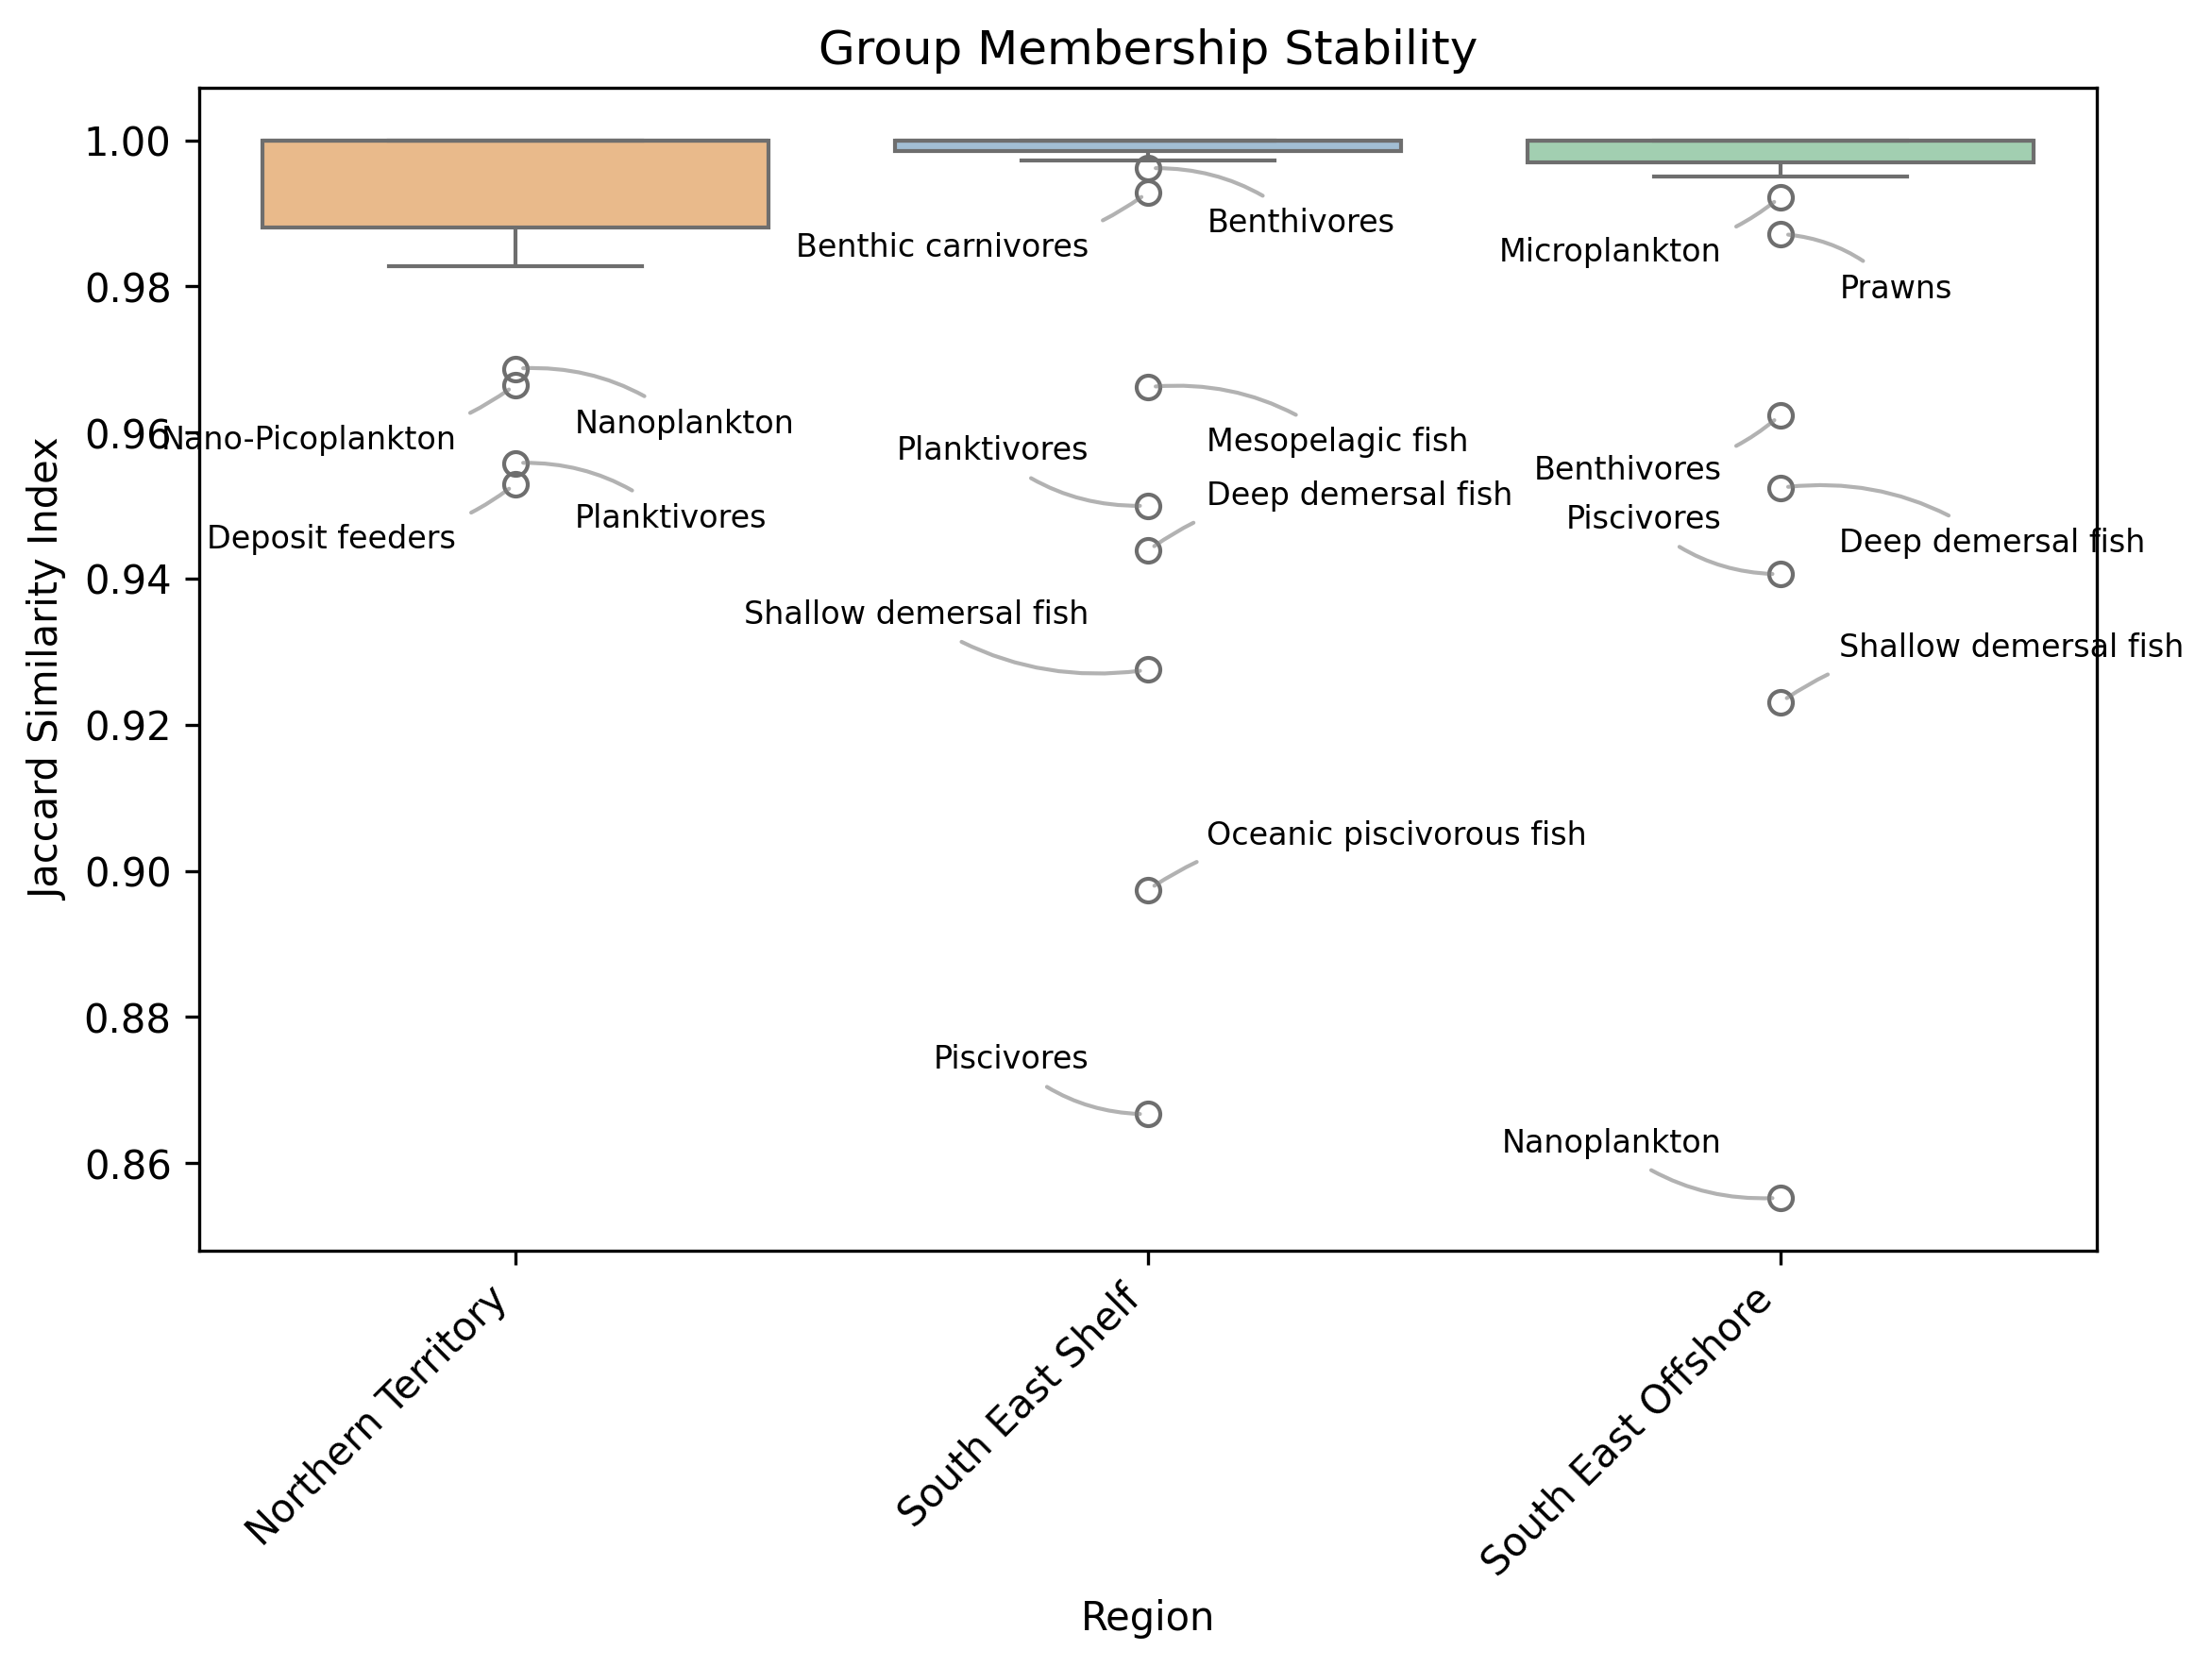
\includegraphics[width=\textwidth]{figures/regional_group_analysis.png}
    \caption{Multi-panel analysis of framework performance across regions. (A) Box plots of functional group sizes (0-3000 species), showing similar median sizes but varying distributions across regions, with outliers indicating some very large groups. (B) Violin plots of species classification consistency (0.4-1.0), where wider sections indicate more species with that consistency score; most species show high consistency (>0.9) with slightly more variation in the Northern Territory. (C) Box plots of group stability measured by Jaccard similarity (0.975-1.000), showing highest stability in South East Offshore and more variable stability in Northern Territory. (D) Box plots of group size variation (standard deviation 0-35), demonstrating larger fluctuations in group membership in the Northern Territory compared to South East regions.}
    \label{fig:regional_analysis}
\end{figure}

\begin{figure}[htbp]
    \centering
    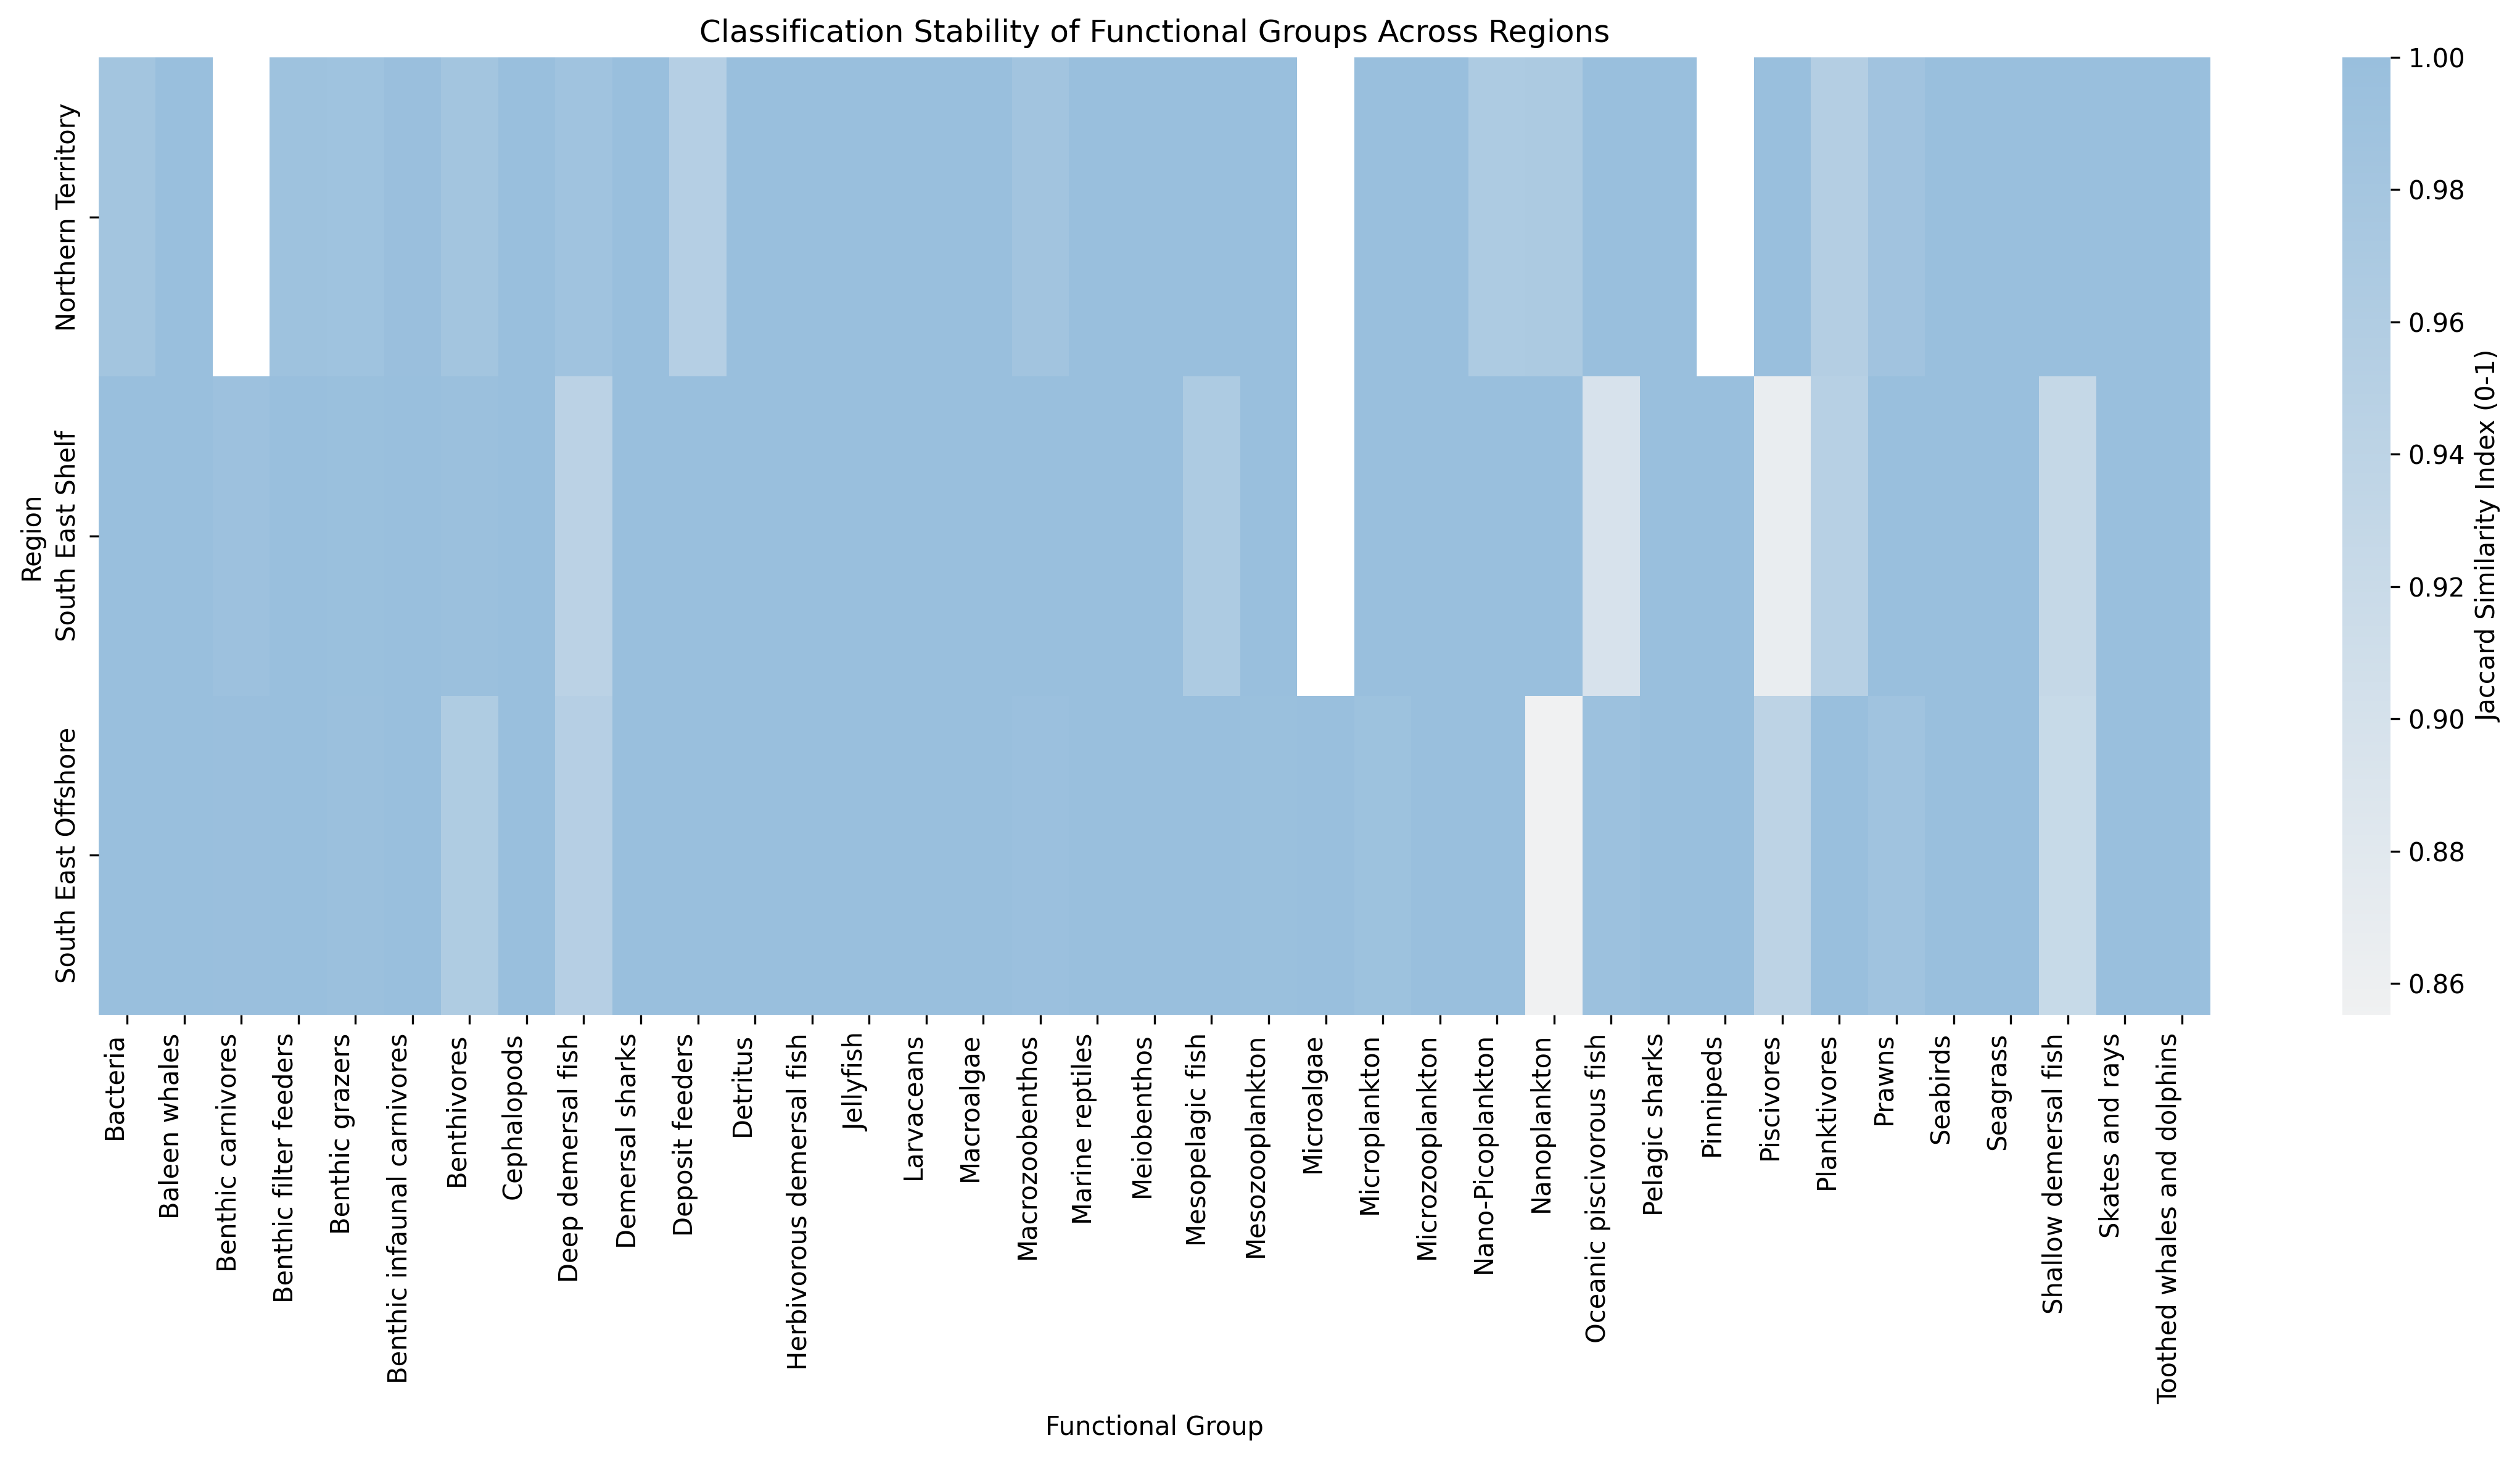
\includegraphics[width=\textwidth]{figures/group_stability_heatmap.png}
    \caption{Heatmap showing the stability of functional group classifications across regions. Each cell displays the Jaccard similarity score (ranging from 0.975 to 1.000) between consecutive framework iterations, where 1.000 indicates perfect consistency in species assignments. Darker red colors represent higher stability (scores near 1.000), while lighter colors indicate more variable classifications (scores closer to 0.975). Most functional groups show high stability (>0.99) across all regions, with occasional variations in groups like benthic grazers and deposit feeders, particularly in the Northern Territory region.}
    \label{fig:stability_heatmap}
\end{figure}

\begin{table}[htbp]
\centering
\caption{Dominant patterns of species classification instability across three study regions. The table presents the most frequent oscillation patterns between functional groups for species that were inconsistently classified across the five framework iterations. For each region, the total number of variably classified species is shown (representing less than 1.1\% of all species), along with the percentage distribution of different oscillation patterns.}
\label{tab:unstable_species}
\small
\begin{tabular}{llcc}
\hline
Region & Most Common Pattern & Count & \% of Total \\
\hline
Northern & Macrozoobenthos $\leftrightarrow$ Benthic infaunal carnivores & 28 & 27.2\% \\
Territory & Benthic filter feeders $\leftrightarrow$ Deposit feeders & 25 & 24.3\% \\
(103 species) & Prawns $\leftrightarrow$ Macrozoobenthos & 21 & 20.4\% \\
& Other patterns & 29 & 28.1\% \\
\hline
South East & Piscivores $\leftrightarrow$ Deep demersal fish & 42 & 33.6\% \\
Inshore & Benthic grazers $\leftrightarrow$ Benthic carnivores & 31 & 24.8\% \\
(125 species) & Planktivores $\leftrightarrow$ Mesopelagic fish & 28 & 22.4\% \\
& Other patterns & 24 & 19.2\% \\
\hline
South East & Benthic filter feeders $\leftrightarrow$ Benthic carnivores & 25 & 28.7\% \\
Offshore & Macrozoobenthos $\leftrightarrow$ Deep demersal fish & 22 & 25.3\% \\
(87 species) & Mesozooplankton $\leftrightarrow$ Macrozoobenthos & 18 & 20.7\% \\
& Other patterns & 22 & 25.3\% \\
\hline
\multicolumn{4}{p{0.95\textwidth}}{\small \textit{Note:} Arrows indicate group assignment oscillation between iterations. Complete species-level data available in Section S3 of the supplementary material.} \\
\hline
\end{tabular}
\end{table}


\subsubsection{Diet Matrix Validation}
The framework demonstrated consistent patterns in diet matrix construction across iterations. Using our stability score metric (where 0 indicates perfect stability and 1 indicates maximum variation), we found that most predator-prey interactions remained highly stable (Figure~\ref{fig:stability_distribution}). The Northern Territory analysis identified 127 predator-prey interactions with a median stability score of 0.18, with 84\% of interactions showing scores below our 0.3 threshold. The South East Inshore region produced 133 interactions with a median stability score of 0.16 (86\% below threshold), while the South East Offshore achieved the highest stability with 147 interactions and a median score of 0.15 (89\% below threshold).

\begin{figure}[htbp]
    \centering
    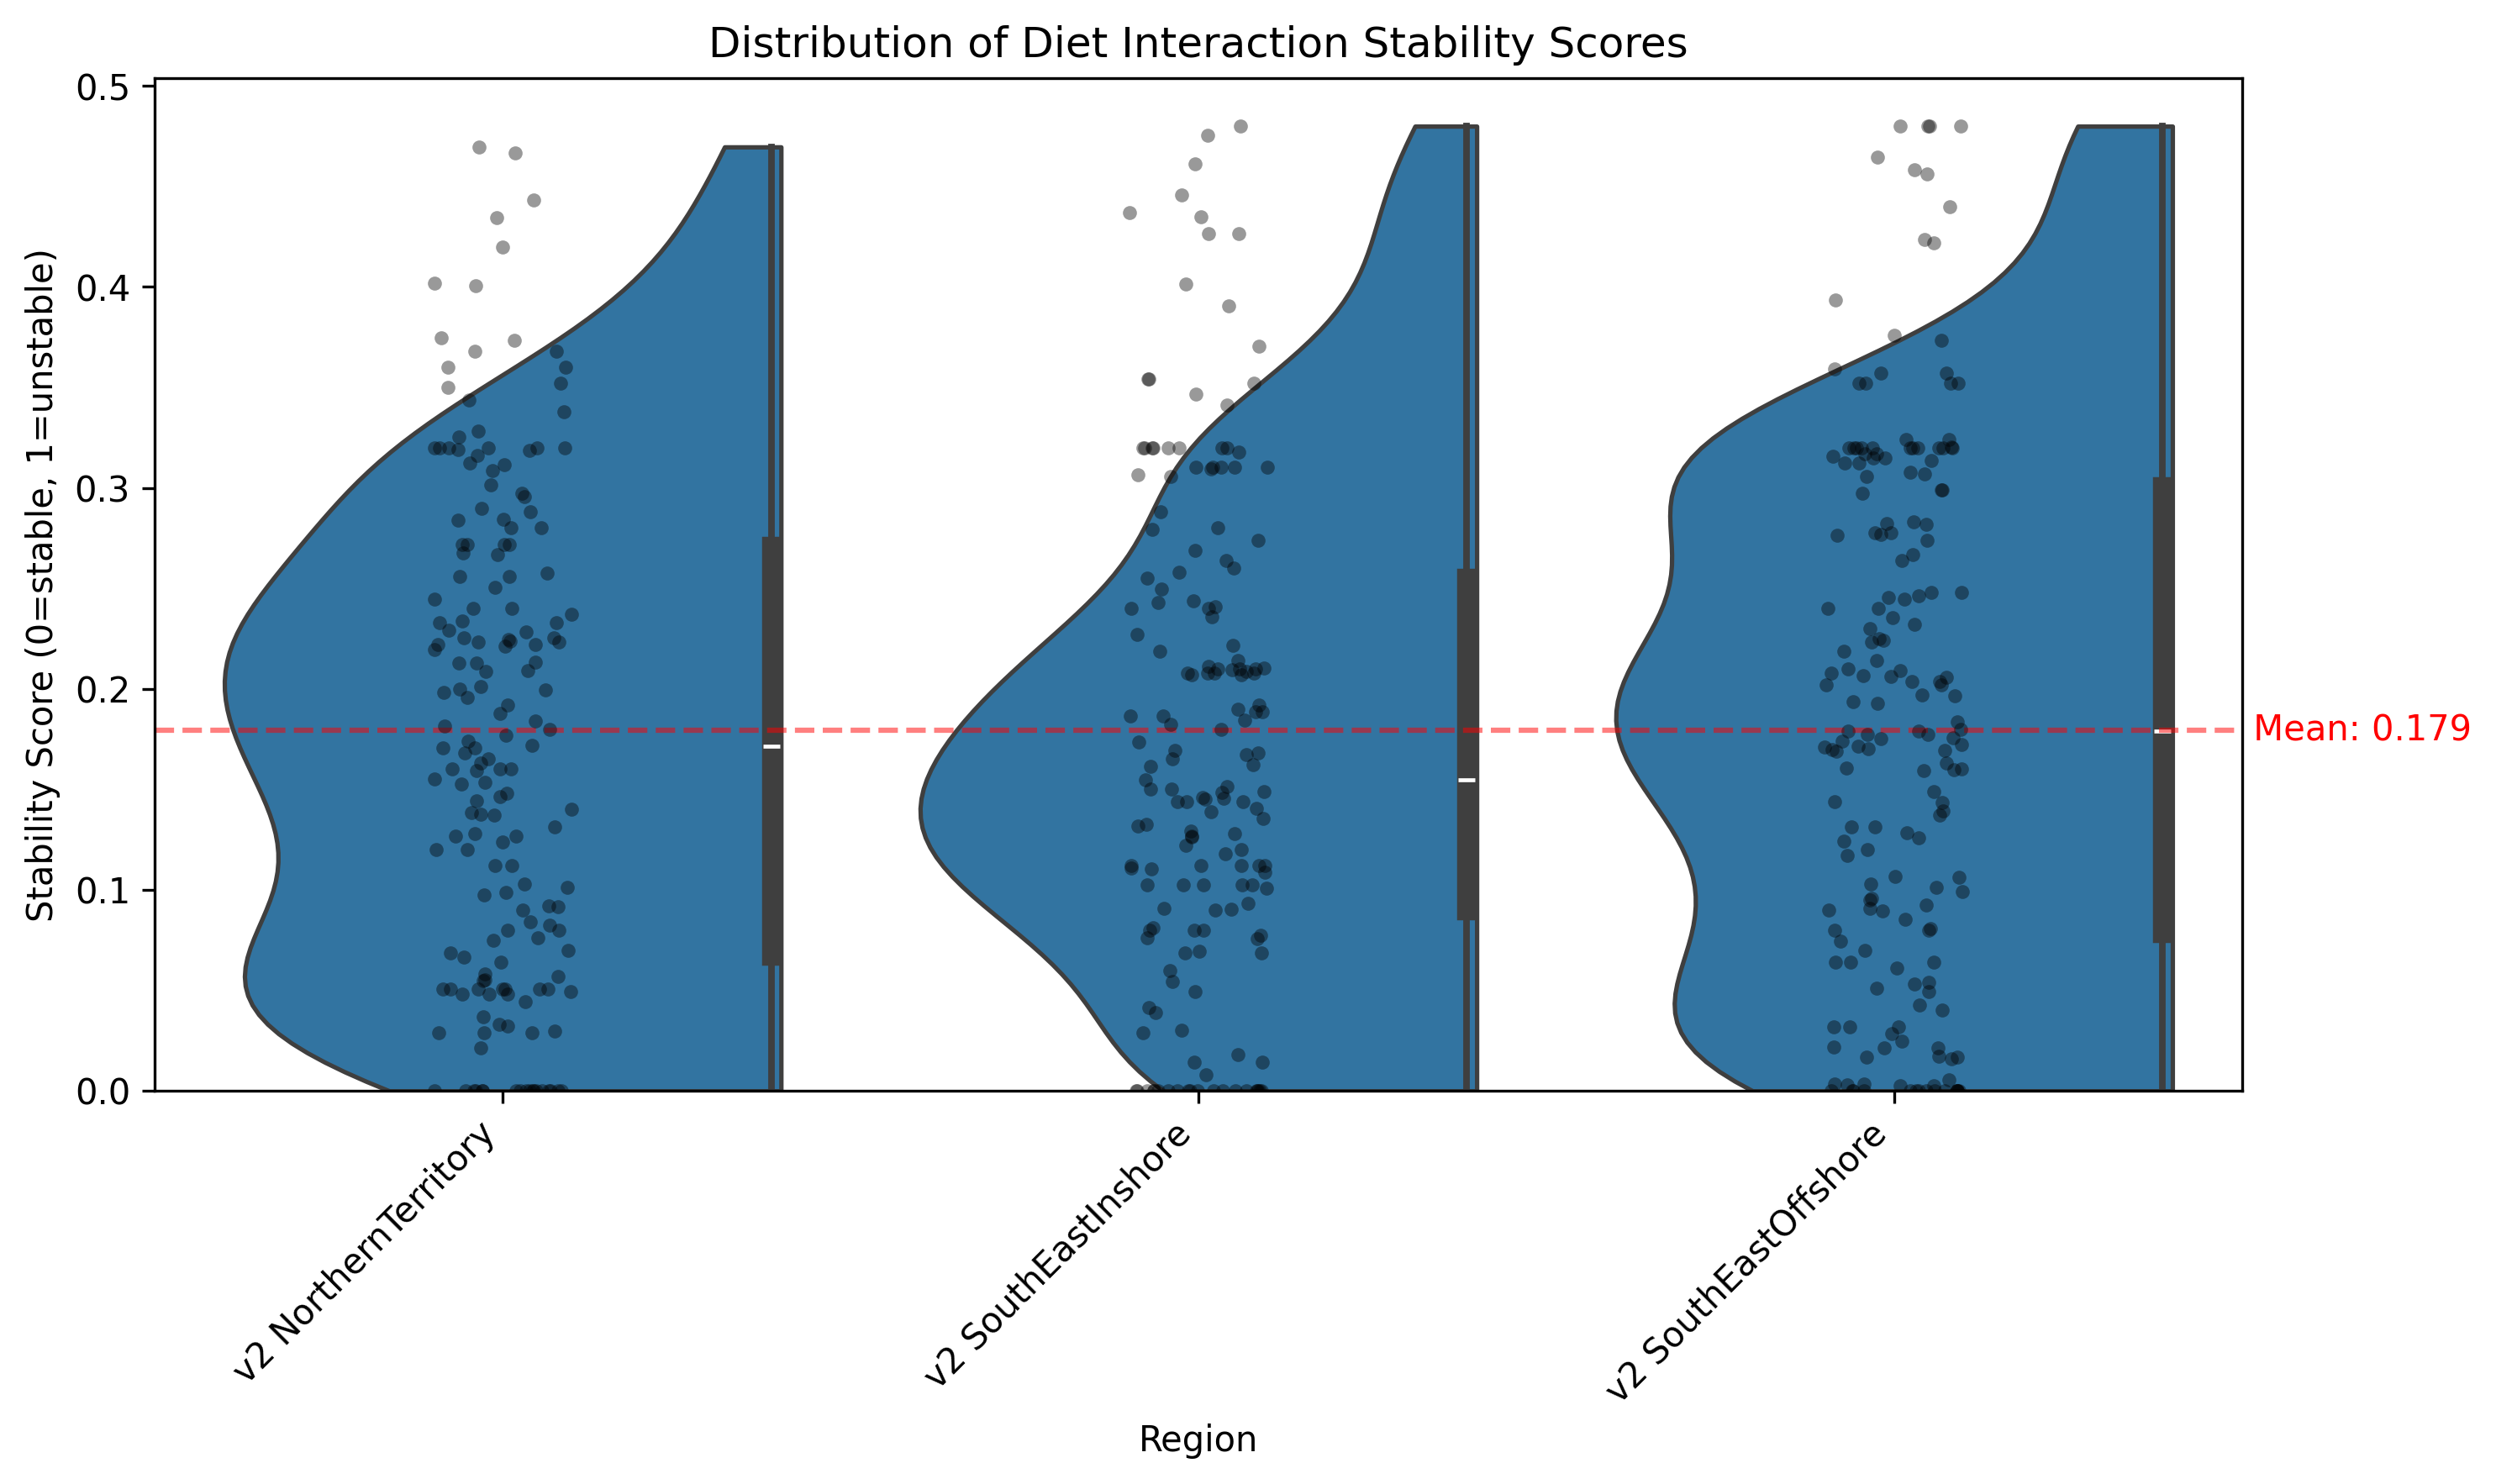
\includegraphics[width=\textwidth]{figures/stability_score_distribution.png}
    \caption{Distribution of diet interaction stability scores across regions. Half-violin plots show the density of stability scores (0=stable, 1=unstable), with embedded box plots indicating quartiles and median. Individual points represent specific predator-prey interactions, and the red dashed line shows the mean stability score across all regions. The distributions are bounded at zero, reflecting perfect stability, with most interactions showing scores below 0.3.}
    \label{fig:stability_distribution}
\end{figure}

Analysis of stability scores by predator group revealed systematic patterns in diet consistency (Figure~\ref{fig:predator_stability}). Lower trophic level groups like nanoplankton and microplankton showed high stability (scores < 0.1) across all regions, reflecting their specialized diets. Mid-trophic level predators such as mesopelagic fish and cephalopods exhibited moderate variability (scores 0.1-0.2), while higher trophic level predators including demersal sharks and benthic carnivores showed the most variation in diet composition (scores > 0.2). This pattern suggests that diet variability increases with trophic level, possibly reflecting the more generalist feeding strategies of higher-level predators. Detailed diet matrices for each region are provided in the supplementary material (Figure~S1).

\begin{figure}[htbp]
    \centering
    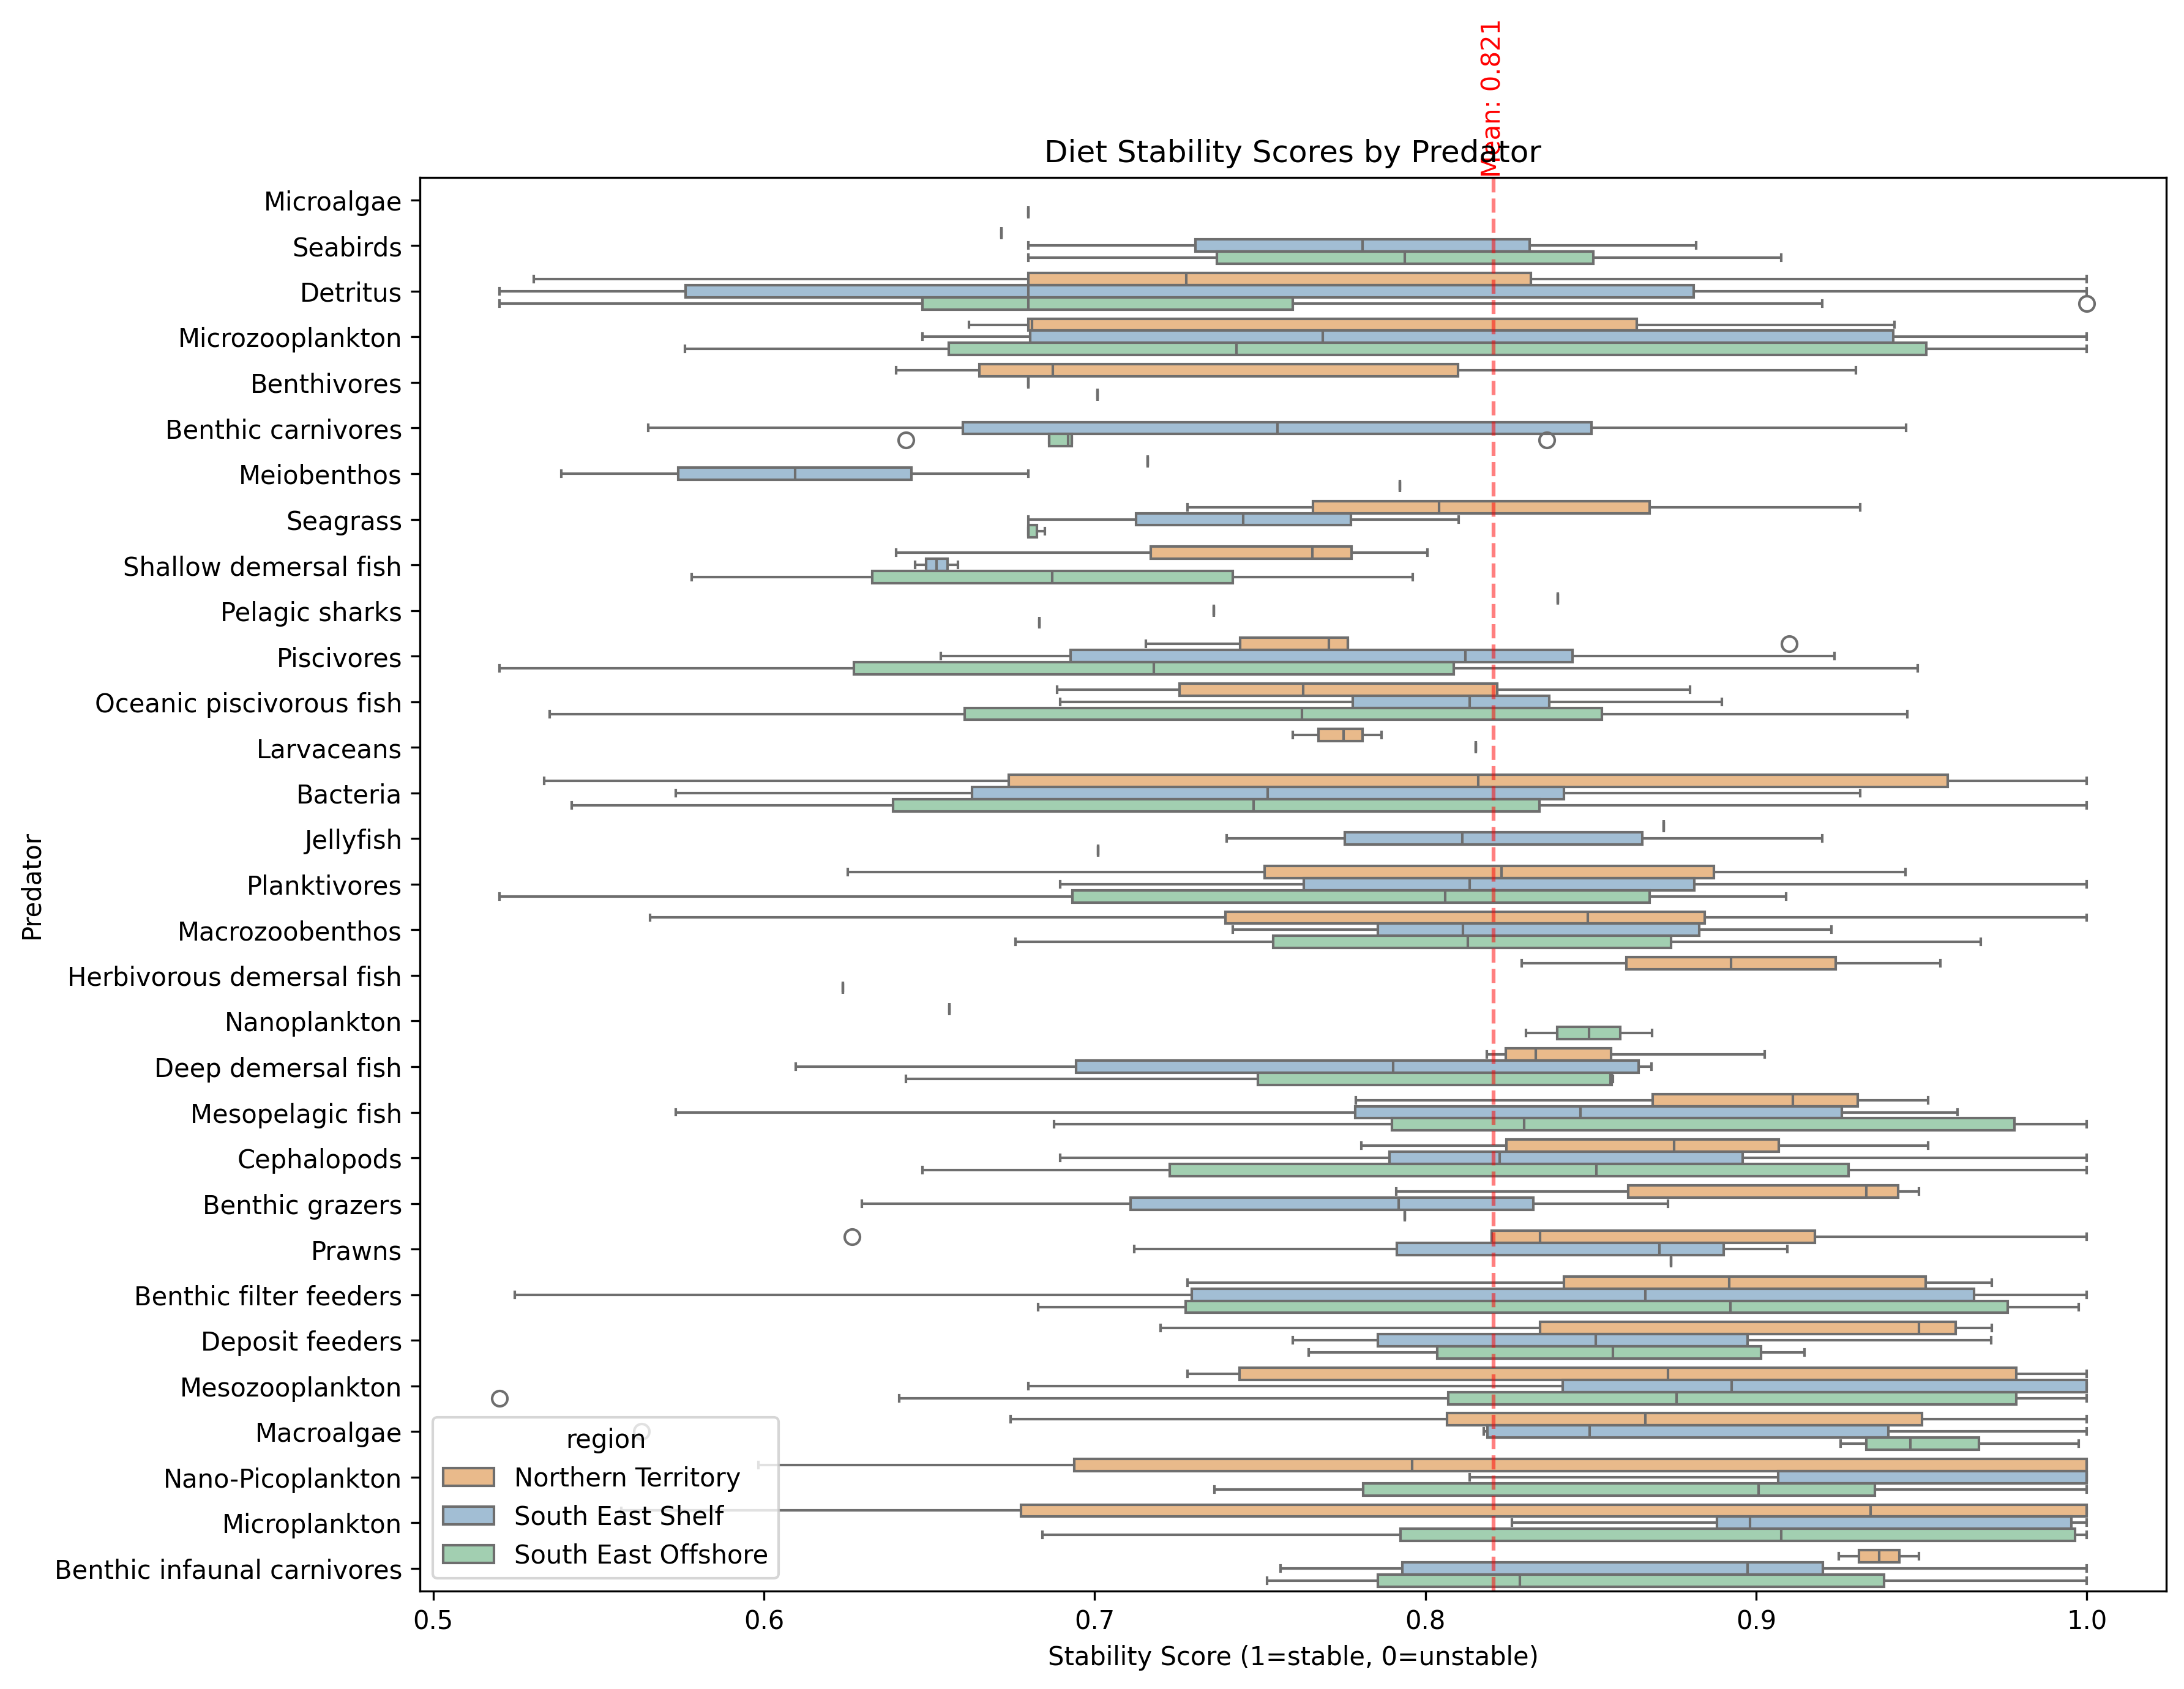
\includegraphics[width=\textwidth]{figures/predator_stability_boxplots.png}
    \caption{Diet stability scores grouped by predator, ordered by median stability. Box plots show the distribution of stability scores for each predator's diet across regions (colored by region). The red dashed line indicates the mean stability score across all predator-prey interactions. Lower scores indicate more consistent diet compositions across framework iterations.}
    \label{fig:predator_stability}
\end{figure}

\subsection{Ecological Findings}

\subsubsection{Trophic Level Patterns}
Analysis of trophic structure revealed significant differences in both the Northern Territory and South East Inshore regions (Kruskal-Wallis H-test, H = 164.0 and 172.0 respectively, p < 0.001 for both). Higher trophic level species, particularly apex predators and specialized feeders, maintained consistent classifications across all regions. In contrast, lower trophic levels showed greater variability, particularly among planktonic and benthic invertebrate groups. Benthivores exhibited the highest variation, ranging from 715 to 788 species between runs, while shallow demersal fish showed moderate variation between 586 and 659 species.
